


\section{Resultados}


\subsection{Experimento 1: Comparación de Métodos de Selección}
En el primer experimento, se comparan tres métodos de selección: ruleta, rango y torneo. Cada método se evalúa utilizando una población de 100 individuos, a lo largo de 3000 generaciones y con una tasa de mutación del 1\%. La función \textbf{'plot\_fitness'} grafica la evolución de la aptitud a lo largo de las generaciones, permitiendo comparar visualmente el desempeño de cada método. Además, la función \textbf{'plot\_route'} muestra la mejor ruta encontrada por cada método.

La siguiente gráfica muestra la evolución de la aptitud a lo largo de las generaciones para cada método de selección:

\begin{figure}[H]
  \centering
  \caption{Comparación de la evolución de la aptitud para los métodos Ruleta, Rango y Torneo}
  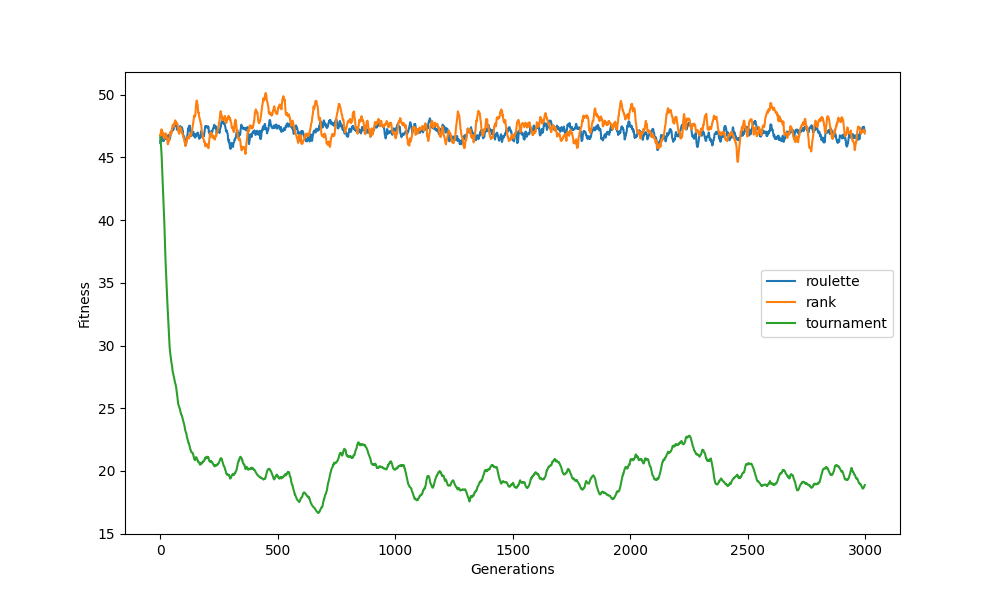
\includegraphics[width=0.8\linewidth]{3_method/Graphs/fitness_comparison_experimento1.png}
\end{figure}

Las mejores rutas encontradas por cada método son las siguientes:

\begin{figure}[H]
  \centering
  \caption{Mejores rutas encontradas por los métodos Ruleta, Rango y Torneo}
  \begin{minipage}{0.32\textwidth}
    \centering
    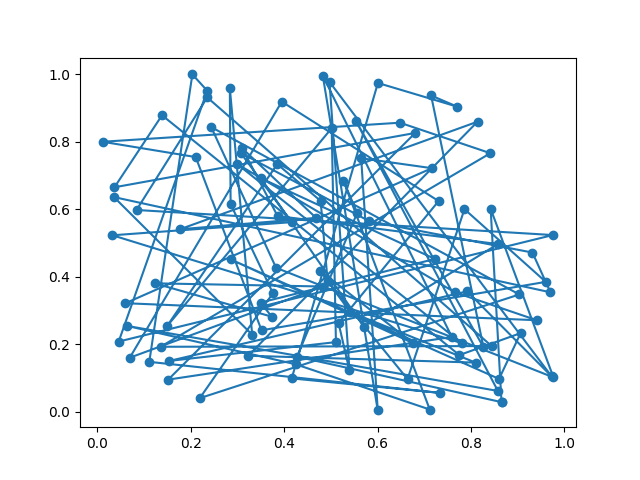
\includegraphics[width=\linewidth]{3_method/Graphs/best_route_(roulette).png}
    \subcaption{Mejor ruta para el método Ruleta}
  \end{minipage}\hfill
  \begin{minipage}{0.32\textwidth}
    \centering
    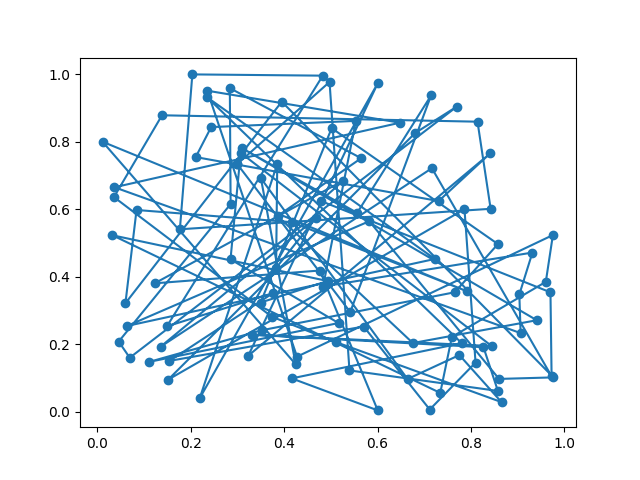
\includegraphics[width=\linewidth]{3_method/Graphs/best_route_(rank).png}
    \subcaption{Mejor ruta para el método Rango}
  \end{minipage}\hfill
  \begin{minipage}{0.32\textwidth}
    \centering
    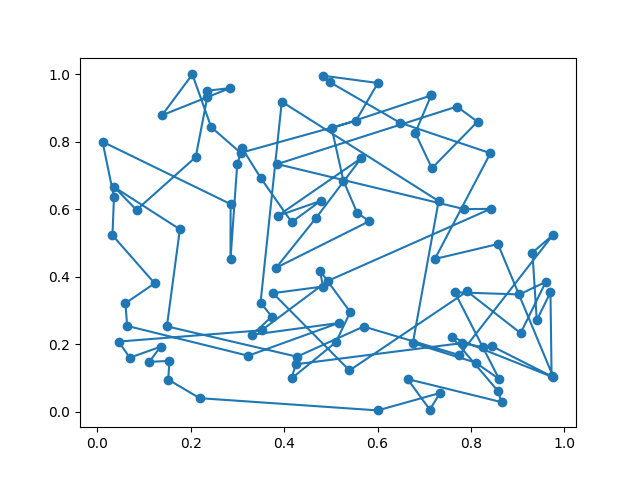
\includegraphics[width=\linewidth]{3_method/Graphs/best_route_(tournament).png}
    \subcaption{Mejor ruta para el método Torneo}
  \end{minipage}
\end{figure}


\subsection{Experimento 2: Comparación de Métodos de Inicialización} 
En el segundo experimento, se comparan tres métodos de inicialización de la población: aleatoria, heurística y una combinación híbrida de ambos. Se utiliza una población de 100 individuos, una tasa de mutación del 1\% y se ejecuta el algoritmo durante 3000 generaciones con selección por torneo. El método de inicialización heurística introduce un componente de conocimiento previo en la generación de los individuos, mientras que el método híbrido busca combinar los beneficios de la aleatoriedad y la heurística. 

La siguiente gráfica muestra la evolución de la aptitud a lo largo de las generaciones para cada método de inicialización:

\begin{figure}[H]
  \centering
  \caption{Comparación de la evolución de la aptitud para los métodos de inicialización Aleatorio, Heurístico e Híbrido}
  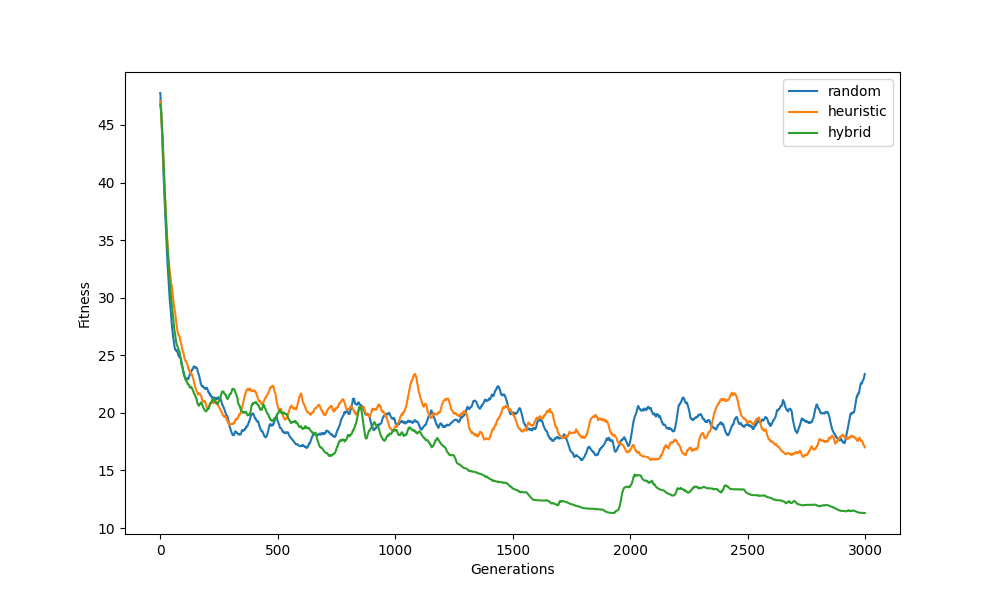
\includegraphics[width=0.8\linewidth]{3_method/Graphs/fitness_comparison_experimento2.png}
\end{figure}

Las mejores rutas encontradas por cada método son las siguientes:


\begin{figure}[H]
  \centering
  \caption{Mejores rutas encontradas por los métodos Aleatorio, Heurístico y Híbrido}
  \begin{minipage}{0.32\textwidth}
    \centering
    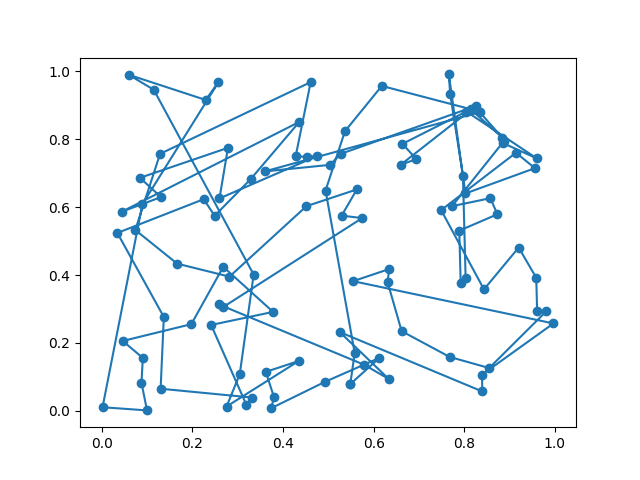
\includegraphics[width=\linewidth]{3_method/Graphs/best_route_(random).png}
    \subcaption{Mejor ruta para el método Aleatorio}
  \end{minipage}\hfill
  \begin{minipage}{0.32\textwidth}
    \centering
    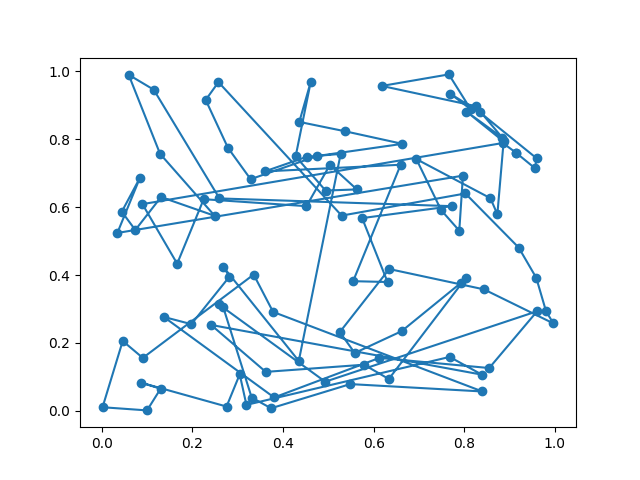
\includegraphics[width=\linewidth]{3_method/Graphs/best_route_(heuristic).png}
    \subcaption{Mejor ruta para el método Heurístico}
  \end{minipage}\hfill
  \begin{minipage}{0.32\textwidth}
    \centering
    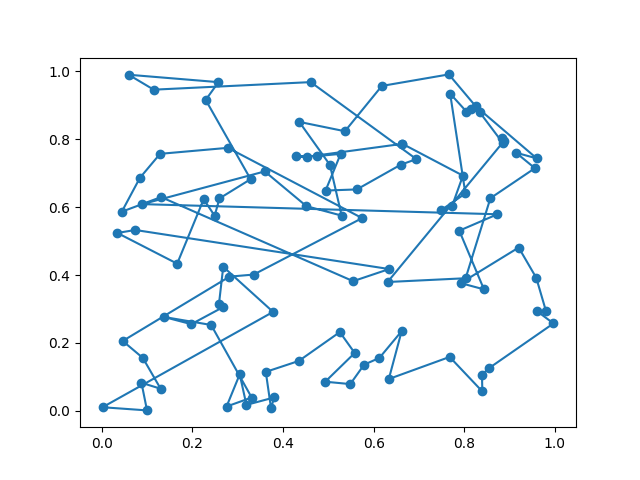
\includegraphics[width=\linewidth]{3_method/Graphs/best_route_(hybrid).png}
    \subcaption{Mejor ruta para el método Híbrido}
  \end{minipage}
\end{figure}
